\chapter{Noise in both models}\label{chap:noise}
\thispagestyle{fancy} %Resets custom page number location on first chapter page

Both benchmarks infer the alignment from noisy observations: zero-mean Gaussian noise is added to every observed PSF (Chapters~\ref{chap:hubble} and~\ref{chap:tma}), while the forward model and the calibration covariances $\boldsymbol{\Sigma}_f$ are noise free. This chapter follows that noise through the pipeline: into the basis coefficients (Section~\ref{sec:noise_model}), into the likelihood explored by nested sampling (Section~\ref{sec:noise_likelihood}) and into the differential-evolution estimate (Section~\ref{sec:noise_de}). It then asks how the results change with the noise level (Section~\ref{sec:noise_sweep}) and how much observations after known moves of the secondary improve the precision (Section~\ref{sec:noise_moves}). The calculations linearize the forward model about the injected truth and are checked against the two pipeline runs and against Monte Carlo simulations.

\section{Noise model and coefficient noise}\label{sec:noise_model}

The observed PSF at each field is $I_{\mathrm{obs}} = I(\boldsymbol{\theta}_{\mathrm{true}}) + n$, where $n$ is independent Gaussian noise with standard deviation $\sigma = 0.01$ in each pixel of the retained image ($64\times64$ pixels for Hubble, $256\times256$ for the TMA). Optiland normalizes the PSF so that an aligned system peaks at 100, so $\sigma$ is $10^{-4}$ of the ideal peak. One noise realization is drawn per field. The noise is additive and independent of the signal, like detector read noise; photon noise, background and other detector effects are not modelled.

Each coefficient is a linear projection of the image onto a basis function $B_k$,
\begin{equation}
c_k = \frac{\langle B_k, I\rangle}{\langle B_k, B_k\rangle},
\end{equation}
where $\langle\cdot,\cdot\rangle$ is the sum over pixels. The pixel noise therefore becomes zero-mean Gaussian noise on the coefficients, with covariance
\begin{equation}
N_{jk} = \sigma^2\,\frac{\langle B_j, B_k\rangle}{\langle B_j, B_j\rangle\,\langle B_k, B_k\rangle}.
\label{eq:noisecov}
\end{equation}
$\mathbf{N}$ is the same at every field and does not depend on $\boldsymbol{\theta}$. For the TMA, the Zernike modes are orthogonal and have equal norm on the unit disk on which they are defined, which covers about $5.1\times10^4$ of the $256\times256$ pixels. Every coefficient therefore has the same noise, $\sigma/\sqrt{5.1\times10^4}=4.4\times10^{-5}$, and the modes are uncorrelated. The circular-Bessel functions used for Hubble are neither normalized nor orthogonal on the $64\times64$ grid: the coefficient noise ranges from $3.0\times10^{-4}$ to $1.1\times10^{-3}$ across the 15 modes, with correlations of up to 0.28 between modes. The Hubble coefficients are also noisier because each projection averages over only 4096 pixels. Table~\ref{tab:noise_coeffs} summarizes these quantities.

\begin{table}
\centering
\caption[Noise in coefficient space, in the likelihood and in the DE objective.]{Noise in coefficient space, in the likelihood and in the DE objective for $\sigma=0.01$ ($10^{-4}$ of the ideal peak). Expected values follow from equation~(\ref{eq:noisecov}); realized values are from the runs in Chapters~\ref{chap:hubble} and~\ref{chap:tma}.}
\label{tab:noise_coeffs}
\begin{tabular}{lll}
\hline
 & \textbf{Hubble} & \textbf{TMA} \\
\hline
Retained image (pixels) & $64\times64$ & $256\times256$ \\
Basis (modes) & circular-Bessel (15) & Zernike (11) \\
Fields; coefficients in total & 5; 75 & 10; 110 \\
Coefficient noise s.d.\ per mode & $(0.3$--$1.1)\times10^{-3}$ & $4.4\times10^{-5}$ \\
Largest noise correlation between modes & 0.28 & $<0.01$ \\
Median $N_{kk}/\Sigma_{f,kk}$ & $1.4\times10^{-5}$ & $6.9\times10^{-5}$ \\
Shift of $-2\ln\mathcal{L}$ at truth, expected & 0.0039 & 0.022 \\
Shift of $-2\ln\mathcal{L}$ at truth, realized & 0.0039 & 0.027 \\
DE cost floor, expected & $(5.3\pm1.0)\times10^{-5}$ & $(2.0\pm0.3)\times10^{-7}$ \\
DE cost, final & $6.2\times10^{-5}$ & $2.2\times10^{-7}$ \\
\hline
\end{tabular}
\end{table}

\section{Effect on the likelihood}\label{sec:noise_likelihood}

The calibration covariances $\boldsymbol{\Sigma}_f$ in the likelihood (equation~\ref{eq:loglike}) come from noise-free Monte Carlo draws of $\boldsymbol{\theta}$, so they describe how much the coefficients vary across the prior, not measurement noise. The noise covariance is tiny by comparison. The diagonal of $\mathbf{N}$ is a median $1.4\times10^{-5}$ (at most $8.1\times10^{-5}$) of the diagonal of $\boldsymbol{\Sigma}_f$ for Hubble, and $6.9\times10^{-5}$ (at most $3.6\times10^{-4}$) for the TMA.

At the truth, the noise $\mathbf{n}_f$ on the observed coefficients raises $-2\ln\mathcal{L}$ by $\sum_f \mathbf{n}_f^{\top}\boldsymbol{\Sigma}_f^{-1}\mathbf{n}_f$, whose expected value is $\sum_f \mathrm{tr}(\boldsymbol{\Sigma}_f^{-1}\mathbf{N})$. This is 0.0039 for Hubble and 0.022 for the TMA. Evaluating the likelihood at the truth in the two runs gives 0.0039 and 0.027. Differences in $\ln\mathcal{L}$ that matter to nested sampling are of order unity, so at this noise level the noise has no material effect on the posteriors in Figures~\ref{fig:hubble_corner} and~\ref{fig:pearl_corner}: their widths are set by $\boldsymbol{\Sigma}_f$. The shift grows as $\sigma^2$ and would reach unity at $\sigma\approx0.16$ for Hubble and $\sigma\approx0.07$ for the TMA. For the TMA, nested sampling and DE used separate noise realizations at the same $\sigma$; by the same argument, this has no practical effect on the nested-sampling stage.

The posterior credible intervals are therefore not noise-limited uncertainties. The Hubble $sdx$ and $sdy$ marginals are nearly flat across the $\pm200\,\mu\mathrm{m}$ prior, while the noise alone limits these parameters to $\approx 4\,\mu\mathrm{m}$ (Section~\ref{sec:noise_de}). A likelihood built from $\mathbf{N}$ instead of $\boldsymbol{\Sigma}_f$ would concentrate the posterior around the noise-limited solution, at the cost of a far more sharply peaked likelihood for the sampler to explore. In the present pipeline, nested sampling serves as a global search, and the precision comes from the DE refinement.

\section{Effect on the differential-evolution estimate}\label{sec:noise_de}

DE minimizes the unweighted sum of squared coefficient residuals over all fields, $S(\boldsymbol{\theta}) = \lVert\mathbf{c}(\boldsymbol{\theta}) - \mathbf{c}_{\mathrm{obs}}\rVert^2$, where $\mathbf{c}$ stacks the coefficients of every field (75 for Hubble, 110 for the TMA). Without noise, the minimum is at the truth, where $S=0$; with noise, it moves. Linearizing the forward model about the truth, $\mathbf{c}(\boldsymbol{\theta})\approx\mathbf{c}(\boldsymbol{\theta}_{\mathrm{true}}) + \mathbf{J}\,\delta\boldsymbol{\theta}$, the least-squares estimate and its covariance are
\begin{equation}
\hat{\boldsymbol{\theta}} - \boldsymbol{\theta}_{\mathrm{true}} \approx \mathbf{A}\,\mathbf{n},\qquad
\mathrm{Cov}(\hat{\boldsymbol{\theta}}) = \mathbf{A}\,\mathbf{N}_{\mathrm{all}}\,\mathbf{A}^{\top},\qquad
\mathbf{A} = (\mathbf{J}^{\top}\mathbf{J})^{-1}\mathbf{J}^{\top},
\label{eq:lscov}
\end{equation}
where $\mathbf{n}$ is the stacked coefficient noise and $\mathbf{N}_{\mathrm{all}}$ is block diagonal, with one copy of $\mathbf{N}$ per field. The expected minimum cost is $\mathrm{tr}[(\mathbf{I}-\mathbf{J}\mathbf{A})\,\mathbf{N}_{\mathrm{all}}]$, the noise power left after the fit absorbs the components along the columns of $\mathbf{J}$. We compute $\mathbf{J}$ by central differences at the truth. The steps are $0.2\,\mu\mathrm{m}$ and $2\times10^{-5}$ degrees for Hubble; for the TMA they are $0.5\,\mu\mathrm{m}$, $5\times10^{-6}$ degrees on the primary tilts and $5\times10^{-5}$ degrees on the secondary tilts. Doubling the steps changes $\mathbf{J}$ by less than 1\%.

The expected minimum costs are $(5.3\pm1.0)\times10^{-5}$ for Hubble and $(2.0\pm0.3)\times10^{-7}$ for the TMA, where the uncertainty is the scatter between noise realizations. The DE runs ended at $6.2\times10^{-5}$ and $2.2\times10^{-7}$, within one standard deviation of these values. Both runs therefore reached the noise floor of their objectives. The flat cost after generation $\sim30$ in the Hubble run (Section~\ref{sec:hubble_results}) and the $2.2\times10^{-7}$ final cost of the TMA run are both set by the noise.

\begin{table}
\centering
\caption[Noise-limited precision of the DE estimate compared with the run residuals.]{Noise-limited precision of the DE estimate, $\sqrt{\mathrm{diag}\,\mathrm{Cov}(\hat{\boldsymbol{\theta}})}$ from equation~(\ref{eq:lscov}), compared with the residuals $\boldsymbol{\theta}_{\mathrm{true}}-\mathbf{c}$ of the runs (Tables~\ref{tab:hubble} and~\ref{tab:pearl}); $z$ is their ratio. Translations are in $\mu$m and tilts in degrees.}
\label{tab:noise_params}
\begin{tabular}{llll}
\hline
\textbf{Parameter} & \textbf{Predicted s.d.} & \textbf{Residual} & $\boldsymbol{z}$ \\
\hline
\multicolumn{4}{l}{\textit{Hubble}} \\
sdx & $3.62$ & $-1.55$ & $-0.43$ \\
sdy & $3.96$ & $-3.82$ & $-0.97$ \\
sdz & $0.075$ & $-0.082$ & $-1.09$ \\
stx & $3.8\times10^{-4}$ & $4.1\times10^{-4}$ & $1.07$ \\
sty & $3.6\times10^{-4}$ & $-1.5\times10^{-4}$ & $-0.42$ \\
\hline
\multicolumn{4}{l}{\textit{TMA}} \\
pdx & $11.3$ & $2.55$ & $0.23$ \\
pdy & $8.79$ & $-10.24$ & $-1.16$ \\
pdz & $2.37$ & $-3.63$ & $-1.53$ \\
sdx & $50.3$ & $-46.12$ & $-0.92$ \\
sdy & $48.4$ & $-9.53$ & $-0.20$ \\
sdz & $2.33$ & $-3.53$ & $-1.52$ \\
ptx & $3.4\times10^{-4}$ & $2.3\times10^{-5}$ & $0.07$ \\
pty & $3.5\times10^{-4}$ & $3.7\times10^{-4}$ & $1.05$ \\
stx & $2.7\times10^{-4}$ & $1.9\times10^{-4}$ & $0.72$ \\
sty & $2.9\times10^{-4}$ & $2.8\times10^{-4}$ & $0.95$ \\
\hline
\end{tabular}
\end{table}

Table~\ref{tab:noise_params} compares the predicted standard deviations with the residuals of the two runs. Every residual lies within 1.6 standard deviations of zero. Taking the correlations into account, the squared Mahalanobis distance of the residual vector, $\delta\boldsymbol{\theta}^{\top}\mathrm{Cov}(\hat{\boldsymbol{\theta}})^{-1}\delta\boldsymbol{\theta}$, is 3.8 for Hubble and 4.9 for the TMA, typical values for $\chi^2$ distributions with 5 and 10 degrees of freedom. The residuals in both runs are thus what the noise predicts: DE found the least-squares solution, and the remaining error comes from the noise rather than from the optimizer. The same holds for image quality. Propagating $\mathrm{Cov}(\hat{\boldsymbol{\theta}})$ to the on-axis OPD by Monte Carlo (300 draws) gives a median RMS WFE of $1.2\times10^{-3}$ waves for Hubble (16th--84th percentiles $0.7$--$1.7\times10^{-3}$) and $4.2\times10^{-3}$ waves for the TMA ($2.4$--$6.9\times10^{-3}$). Both ranges contain the $1.35\times10^{-3}$ and $2.5\times10^{-3}$ waves reached by the runs.

The noise-limited errors are not spread evenly across the parameters: they concentrate along the same near-degeneracies that shape the posteriors (Figure~\ref{fig:noise_ellipses}). For Hubble, the decenter errors are almost perfectly correlated with the secondary tilt about the perpendicular axis ($r=-0.996$ for $sdy$--$stx$ and $r=+0.995$ for $sdx$--$sty$). A decenter and a tilt of the secondary both introduce nearly field-constant coma, the mechanism described for the TMA in Section~\ref{sec:pearl_results}, so one can largely compensate the other. If all the other parameters were known, the noise would determine $sdx$ and $sdy$ to $0.36$ and $0.32\,\mu\mathrm{m}$ instead of $3.6$ and $4.0\,\mu\mathrm{m}$. For the TMA, the strongest correlations are $pdz$--$sdz$ ($r=1.00$), $pty$--$sty$ ($0.99$), $sdx$--$sty$ ($-0.98$), $sdy$--$ptx$ ($0.98$) and $sdx$--$pty$ ($-0.98$), which include the pairs found in the TMA posterior. If the other nine parameters were known, the noise alone would determine $sdx$ to $0.30\,\mu\mathrm{m}$; the degeneracies amplify this to $50\,\mu\mathrm{m}$. The large $sdx$ residual of the TMA run ($46\,\mu\mathrm{m}$) is therefore noise projected onto a nearly degenerate direction, and the near-unity $pdz$--$sdz$ correlation is the focus trade-off between the two despaces.

\begin{figure}
    \centering
    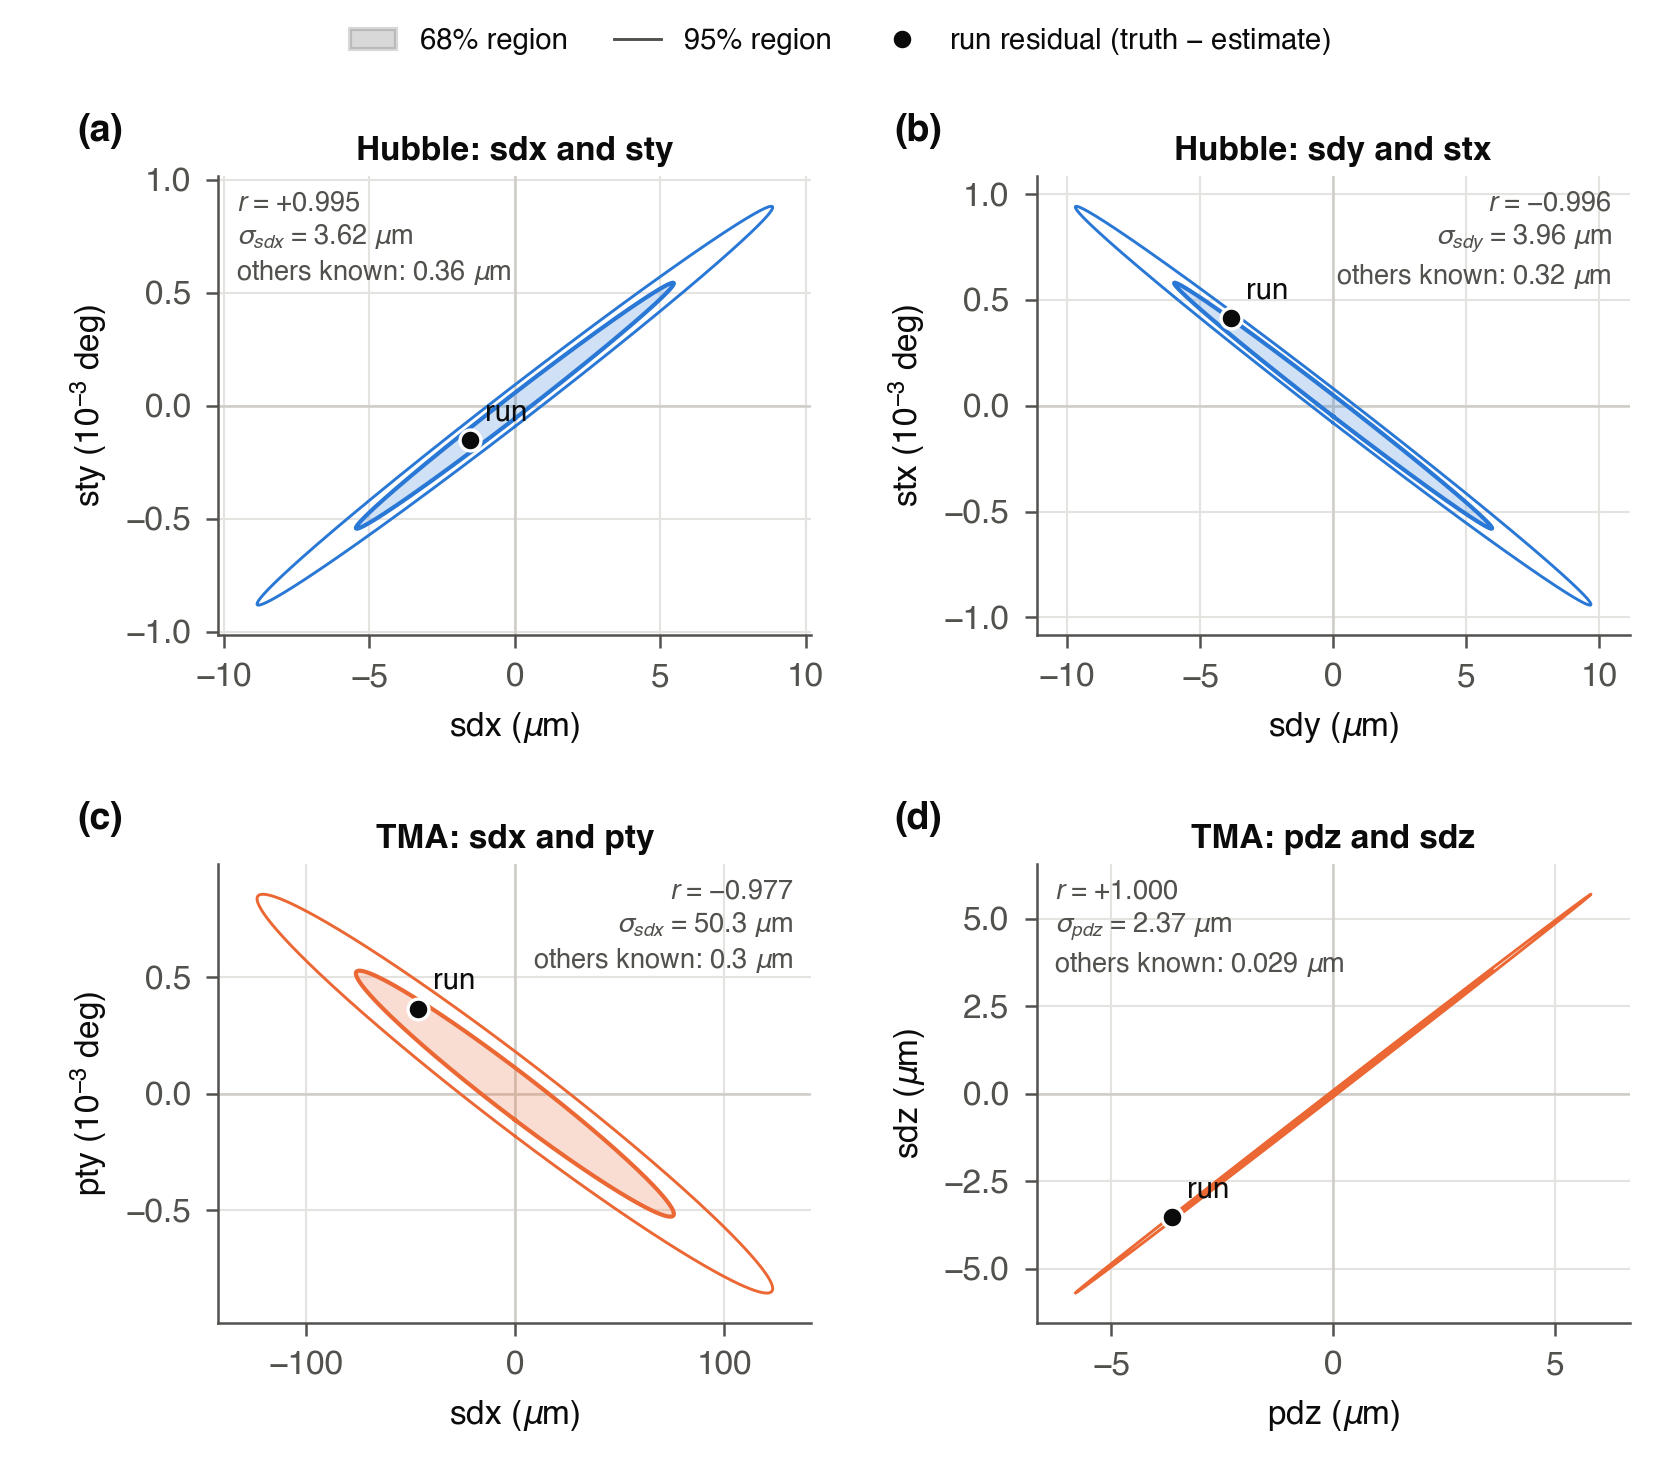
\includegraphics[width=0.85\textwidth]{figures/noise_ellipses.png}
    \caption[Noise-limited scatter of the DE estimate along the strongest correlations.]{Noise-limited scatter of the DE estimate in the planes of the strongest correlations: the 68\% and 95\% regions of the linearized covariance (equation~\ref{eq:lscov}) for Hubble (a, b; blue) and the TMA (c, d; orange), with the residual $\boldsymbol{\theta}_{\mathrm{true}}-\mathbf{c}$ of each run (black). Tilts are in $10^{-3}$ degrees. Each panel gives the correlation coefficient, the standard deviation of the horizontal parameter, and its standard deviation if all other parameters were known.}
    \label{fig:noise_ellipses}
\end{figure}

Because the circular-Bessel coefficient noise is unequal across modes and correlated, weighting the DE objective by $\mathbf{N}^{-1}$ (generalized least squares) would give the minimum-variance estimate. For Hubble, this would reduce the predicted standard deviations by only 5--13\%. For the TMA, $\mathbf{N}$ is proportional to the identity, so weighting would change nothing.

The noise-free limit is consistent with this picture. In an earlier noise-free run of the Hubble benchmark, with an on-axis DE objective, DE reached an objective below $10^{-15}$ and recovered the translations to better than $0.01\,\mu\mathrm{m}$, with an on-axis OPD RMS of $\sim3\times10^{-8}$ waves.

\section{Dependence on noise level}\label{sec:noise_sweep}

In the linear approximation, the parameter errors and the WFE scale in proportion to $\sigma$: the values for another noise level follow by multiplying those in Table~\ref{tab:noise_params} by $\sigma/0.01$. To test where this breaks down, we simulated noisy observations at the truth for $\sigma = 0.01$, 0.03, 0.1 and 0.3 ($10^{-4}$ to $3\times10^{-3}$ of the ideal peak), with 50 realizations per level for Hubble and 30 for the TMA. Each least-squares problem was solved from the truth with twelve Gauss--Newton iterations, holding $\mathbf{J}$ at its value at the truth; in spot checks, the final steps were below $10^{-3}$ of the predicted standard deviation. The simulations start from the truth and ignore the DE bounds, so they describe the least-squares solution nearest the truth rather than every solution DE might return. Table~\ref{tab:noise_sweep} and Figure~\ref{fig:noise_sweep} compare the RMS errors and the median WFE of these solutions with the linear predictions.

\begin{figure*}
    \centering
    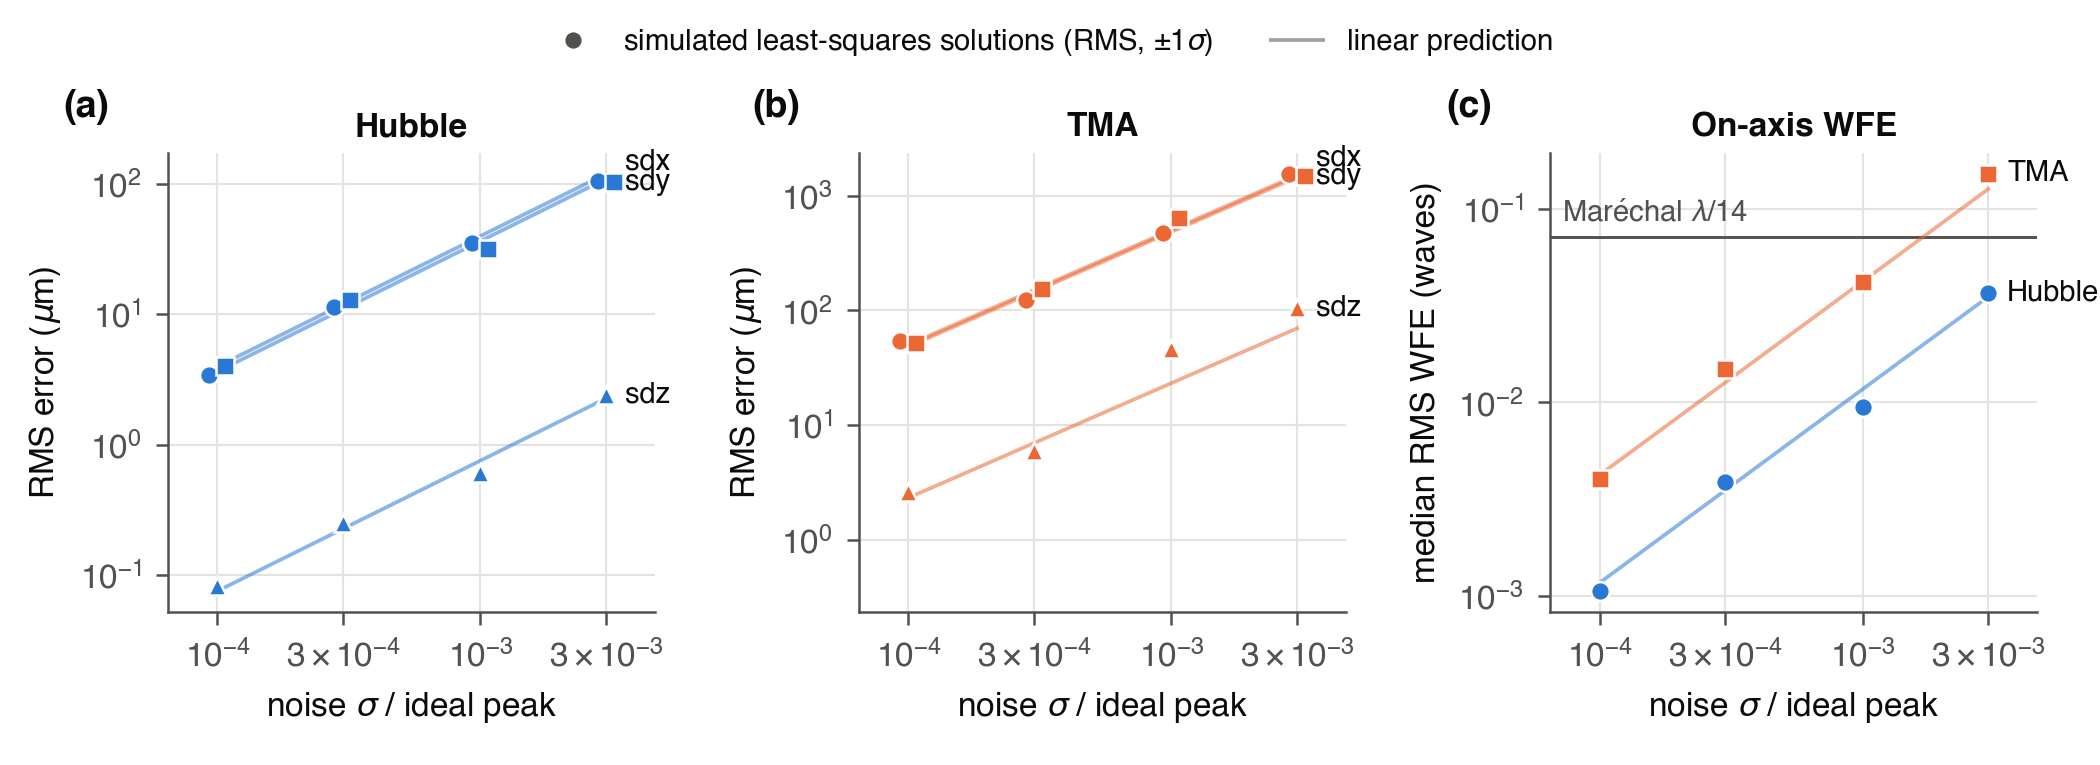
\includegraphics[width=\textwidth]{figures/noise_sweep.png}
    \caption[Parameter errors and on-axis WFE versus noise level.]{Parameter errors and on-axis WFE versus noise level. (a, b) RMS errors of the secondary decenters and despace for Hubble and the TMA. Points are simulated least-squares solutions (50 and 30 noise realizations per level for Hubble and the TMA; error bars show the $\pm1\sigma$ uncertainty of each RMS value), and lines are the linear prediction, proportional to $\sigma$. The $sdx$ and $sdy$ points are offset slightly along $\sigma$ so that both are visible. The TMA $pdz$ errors (Table~\ref{tab:noise_sweep}) follow $sdz$. (c) Median on-axis RMS WFE of the same solutions, with the Mar{\'e}chal criterion $\lambda/14$.}
    \label{fig:noise_sweep}
\end{figure*}

\begin{table}
\centering
\small
\caption[Parameter errors and WFE versus noise level.]{RMS parameter errors and median on-axis RMS WFE of simulated least-squares solutions at four noise levels, with the linear prediction in parentheses. $\sigma=0.01$ in Optiland units is $10^{-4}$ of the ideal peak. With 50 (Hubble) and 30 (TMA) realizations per level, the simulated RMS values are uncertain by about 10\% and 13\%.}
\label{tab:noise_sweep}
\begin{tabular}{lllllll}
\hline
 & \multicolumn{3}{c}{\textbf{Hubble}} & \multicolumn{3}{c}{\textbf{TMA}} \\
$\sigma/I_{\mathrm{peak}}$ & sdx ($\mu$m) & sdy ($\mu$m) & WFE ($10^{-3}$) & sdx ($\mu$m) & pdz ($\mu$m) & WFE ($10^{-3}$) \\
\hline
$10^{-4}$ & 3.41 (3.62) & 4.01 (3.96) & 1.06 (1.17) & 53.7 (50.3) & 2.67 (2.37) & 4.02 (4.22) \\
$3\times10^{-4}$ & 11.3 (10.9) & 12.9 (11.9) & 3.89 (3.51) & 123 (151) & 6.09 (7.12) & 14.9 (12.6) \\
$10^{-3}$ & 35.0 (36.2) & 31.6 (39.6) & 9.49 (11.7) & 472 (503) & 46.9 (23.7) & 41.8 (42.2) \\
$3\times10^{-3}$ & 105 (109) & 102 (119) & 36.7 (35.1) & 1550 (1510) & 107 (71.2) & 152 (126) \\
\hline
\end{tabular}
\end{table}

For Hubble, the simulated errors and WFE follow the linear prediction to within about 20\% at every level, so the linear scaling holds up to at least $\sigma=0.3$. The median WFE there, 0.037 waves, is still within the Mar{\'e}chal criterion of $\lambda/14\approx0.071$ waves. For the TMA, the linear prediction holds for $\sigma\le0.03$. At $\sigma=0.1$, the despace errors are twice the linear prediction ($47\,\mu\mathrm{m}$ on $pdz$ against $24\,\mu\mathrm{m}$), as the $pdz$--$sdz$ trade-off is no longer linear. At $\sigma=0.3$, the median WFE of 0.15 waves is 20\% above the linear value and exceeds the Mar{\'e}chal criterion; the linear prediction places the crossing near $\sigma\approx0.17$, or $0.17\%$ of the ideal peak. At that level, the RMS error in the TMA secondary decenters ($\approx1.5$\,mm) is comparable to the half-width of the DE bounds used in Chapter~\ref{chap:tma}.

\section{Observations after known moves of the secondary}\label{sec:noise_moves}

Section~\ref{sec:noise_de} showed that the Hubble DE estimate is limited by the observation noise, amplified along the decenter--tilt degeneracy. There are two ways to raise its precision: collect more light, which reduces every error as $1/\sqrt{M}$ for $M$ exposures, or make the observations themselves more informative. Phase diversity~\citep{Gonsalves1982} does the latter by recording a second image with a known added aberration, usually defocus. The alignment mechanism can provide the added aberration itself: the secondary is moved by known amounts relative to its unknown position, and the PSFs are recorded again at each position. This section asks how much such moves improve the Hubble estimate, first with the linearized analysis of Section~\ref{sec:noise_de} and then with full runs of the pipeline for two move sizes.

If the secondary is observed at $\boldsymbol{\theta}_{\mathrm{true}}+\boldsymbol{\delta}_m$, $m=0,\dots,M-1$, with $\boldsymbol{\delta}_0=\mathbf{0}$ and every $\boldsymbol{\delta}_m$ known, the DE objective (equation~\ref{eq:de_cost}) becomes a sum over positions,
\begin{equation}
S(\boldsymbol{\theta}) = \sum_{m=0}^{M-1}\sum_{f\in\mathcal{F}}\sum_{k=1}^{N_z}\left[c_{f,k}(\boldsymbol{\theta}+\boldsymbol{\delta}_m) - c_{m,f,k,\mathrm{obs}}\right]^2,
\label{eq:de_cost_moves}
\end{equation}
and equation~(\ref{eq:lscov}) becomes
\begin{equation}
\mathrm{Cov}(\hat{\boldsymbol{\theta}}) =
\Bigl(\sum_{m}\mathbf{J}_m^{\top}\mathbf{J}_m\Bigr)^{-1}
\Bigl(\sum_{m}\mathbf{J}_m^{\top}\mathbf{N}_{\mathrm{all}}\mathbf{J}_m\Bigr)
\Bigl(\sum_{m}\mathbf{J}_m^{\top}\mathbf{J}_m\Bigr)^{-1},
\label{eq:lscov_moves}
\end{equation}
where $\mathbf{J}_m$ is the Jacobian of the coefficients of all fields at $\boldsymbol{\theta}_{\mathrm{true}}+\boldsymbol{\delta}_m$ and $\mathbf{N}_{\mathrm{all}}$ is as before. If every $\boldsymbol{\delta}_m$ is zero, the $M$ exposures are repeats, all $\mathbf{J}_m$ are equal and every standard deviation falls by $\sqrt{M}$. The benefit of moving is therefore measured against the same number of exposures at the nominal position: we define the gain as the standard deviation from $M$ such exposures divided by the standard deviation with the moves.

\begin{figure*}
    \centering
    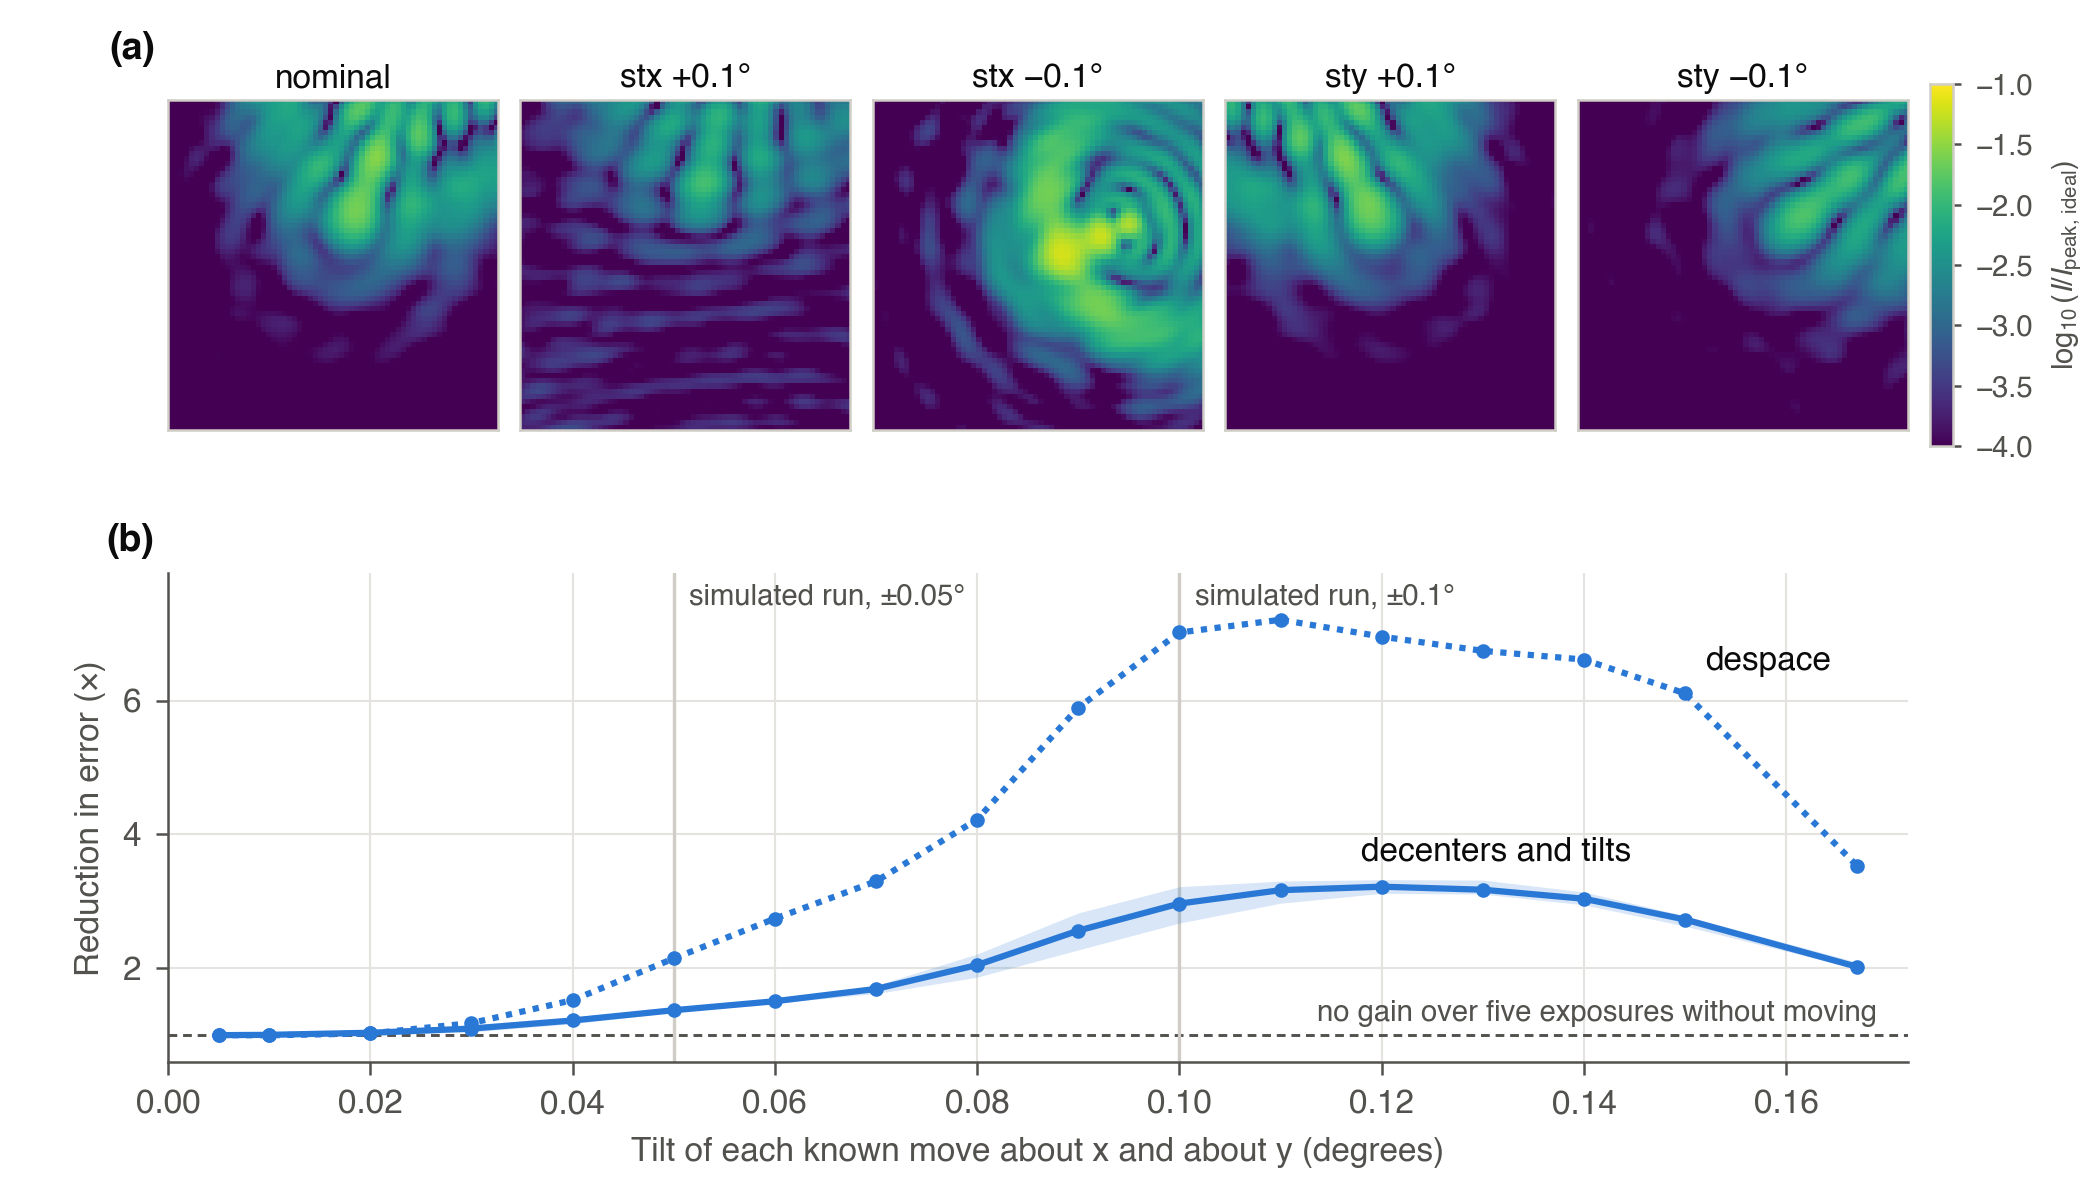
\includegraphics[width=\textwidth]{figures/noise_moves.png}
    \caption[Known moves of the Hubble secondary.]{Known moves of the Hubble secondary. (a) On-axis PSF, on a logarithmic scale relative to the ideal peak, at the injected misalignment and after the four known tilts of $\pm0.1$ degrees used in the first simulation. (b) Predicted reduction in the noise-limited error of the DE estimate relative to five exposures at the nominal position (equation~\ref{eq:lscov_moves}), for five positions: the nominal one and tilts of $\pm\Delta$ about $x$ and about $y$. The band spans the four decenter and tilt parameters and the solid line is their mean; the dotted line is the despace. The vertical lines mark the two simulated designs.}
    \label{fig:noise_moves}
\end{figure*}

Figure~\ref{fig:noise_moves}b shows the gain for designs of five positions: the nominal one and tilts of $\pm\Delta$ about $x$ and about $y$. Moves of $0.01$ degrees or less give no gain, and moves of $0.02$ degrees at most 7\%. The PSF responds almost linearly to such small changes, so a moved PSF carries nearly the same information as a repeated exposure, and the improvement is essentially the factor $\sqrt{5}$ from five times the exposure. The gain rises from about $0.03$ degrees, peaks near $0.11$--$0.12$ degrees at 3.1--3.3 on the decenters and tilts and 7.2 on the despace, and falls for larger moves, possibly because these push the PSF toward the edge of the $64\times64$-pixel cutout (Figure~\ref{fig:noise_moves}a). What matters is the amount of known coma a move adds rather than the actuator that makes it. In coma, one degree of secondary tilt is equivalent to about $10$\,mm of decenter, and decenter moves matched in coma give similar gains: 2.3--2.7 on the decenters and tilts for $\pm1$\,mm, but none for $\pm100$--$200\,\mu\mathrm{m}$. Moves in despace mainly improve the despace estimate (by $1.9$ for $\pm100\,\mu\mathrm{m}$, against at most $1.2$ for the other parameters), and moves of $\pm400\,\mu\mathrm{m}$ degrade every parameter.

To test the prediction, we repeated the Hubble benchmark of Chapter~\ref{chap:hubble} twice, keeping the injected misalignment: with the nominal position and tilts of $\pm0.1$ degrees about $x$ and about $y$, close to the predicted optimum, and with tilts of $\pm0.05$ degrees, for which the predicted gain from the moves is only 1.3--2.2. Each of the five positions was observed at the five fields of Section~\ref{sec:hubble} with independent noise ($\sigma=0.01$), giving 25 PSFs and 375 coefficients per run; the two runs share the same noise draws. The likelihood (equation~\ref{eq:loglike}) and the DE objective (equation~\ref{eq:de_cost_moves}) sum over the positions. Each moved position uses the calibration covariance $\boldsymbol{\Sigma}_f$ of its field; this is an approximation, but a $0.1$-degree move lies well within the distribution from which $\boldsymbol{\Sigma}_f$ was estimated. The noise realization differs from that of Chapter~\ref{chap:hubble}. Since an evaluation now needs 25 PSFs, the five positions were computed in parallel, which kept the time per evaluation close to that of the nominal run.

With tilts of $\pm0.1$ degrees, Nautilus needed $75\,400$ likelihood evaluations ($N_{\mathrm{eff}}\approx1.6\times10^4$). Unlike the nominal run, whose $sdx$ and $sdy$ marginals are nearly flat (Figure~\ref{fig:hubble_corner}), the posterior concentrates on a lattice of modes about $100\,\mu\mathrm{m}$ apart in $sdx$ and $sdy$, the highest of which contains the truth. The lattice comes from the prior transform, which rounds the tilts to $0.01$ degrees (Section~\ref{sec:prior_like}): a tilt step of $0.01$ degrees is compensated by about $100\,\mu\mathrm{m}$ of decenter, so each neighbouring tilt value produces its own mode. The weighted median of the final 100 posterior samples was $(53.17,\allowbreak\,-114.35,\allowbreak\,39.05,\allowbreak\,0.13,\allowbreak\,-0.04)$, within $1\,\mu\mathrm{m}$ of the truth on both decenters, compared with $113\,\mu\mathrm{m}$ on $sdy$ in the nominal run. Its on-axis WFE, $1.9\times10^{-3}$ waves, is already close to the final result of the nominal run. Because the tilt posterior is narrower than the rounding step, nearly all of the weight of the final 100 samples lies on the true tilt values, and the 2.1\%--97.9\% DE bounds on $stx$ and $sty$ collapse to single values. SciPy holds a parameter with equal bounds fixed, so we widened each collapsed bound by one rounding step on each side, to $(0.12,\,0.14)$ and $(-0.05,\,-0.03)$ degrees.

With tilts of $\pm0.05$ degrees, Nautilus needed $60\,900$ evaluations ($N_{\mathrm{eff}}\approx1.4\times10^4$). The posterior shows the same lattice of modes, but the modes carry similar weight, and most of the weight of each tilt is spread over three grid values, $0.11$--$0.13$ and $-0.05$ to $-0.03$ degrees. No bound collapsed, and the DE bounds on the decenters stayed wide, $220\,\mu\mathrm{m}$ on $sdx$ and $125\,\mu\mathrm{m}$ on $sdy$ (against 327 and $378\,\mu\mathrm{m}$ in the nominal run). The weighted median of the final 100 samples, $(51.05,\allowbreak\,-111.11,\allowbreak\,39.15,\allowbreak\,0.13,\allowbreak\,-0.04)$, was still within $3\,\mu\mathrm{m}$ of the truth on both decenters, with an on-axis WFE of $5.2\times10^{-3}$ waves.

In both runs DE used deferred updating, as in the TMA run, so that each generation could be evaluated in parallel. In the $\pm0.1$-degree run, its cost came within 1\% of its final value by generation 47, and the run was stopped by hand after 137 generations at $S=2.78\times10^{-4}$. The expected minimum of the five-position objective is $(2.84\pm0.23)\times10^{-4}$, so the run reached the noise floor; L-BFGS-B polishing left the solution unchanged. Table~\ref{tab:noise_moves} compares the residuals with the predicted standard deviations. For this run, every residual lies within 0.9 standard deviations of zero, and the squared Mahalanobis distance of the residual vector is 2.9, a typical value for five degrees of freedom. The predicted standard deviations are 6.0--7.2 times smaller than for the nominal position alone on the decenters and tilts and 16 times smaller on the despace. Of these factors, $\sqrt{5}\approx2.2$ comes from the additional exposures and 2.7--3.2 (7.0 on the despace) from the moves. Image quality improves accordingly. Propagating the covariance to the on-axis OPD by Monte Carlo (300 draws) gives a median RMS WFE of $1.5\times10^{-4}$ waves (16th--84th percentiles $0.8$--$2.4\times10^{-4}$), against $1.2\times10^{-3}$ waves for the nominal position. The run reached $2.1\times10^{-4}$ waves, compared with $1.35\times10^{-3}$ waves in Chapter~\ref{chap:hubble}.

The $\pm0.05$-degree run was given its full 1000 generations. Its cost came within 1\% of its final value by generation 48 and within 0.1\% by generation 70, ending at $2.75\times10^{-4}$ against an expected $(2.83\pm0.23)\times10^{-4}$; polishing moved the estimate by less than $10^{-7}$. Its residuals lie between 1.0 and 1.7 standard deviations from zero, larger than in the $\pm0.1$-degree run but consistent with the noise. They come in pairs along the two degenerate directions, $sdy$ with $stx$ ($z=-1.54$ and $+1.54$) and $sdx$ with $sty$ ($z=-1.70$ and $-1.63$), and the squared Mahalanobis distance of the residual vector, 5.4, is again typical for five degrees of freedom. The predicted standard deviations are 3.0--3.1 times smaller than for the nominal position alone on the decenters and tilts and 4.8 times smaller on the despace. Of these factors, $\sqrt{5}$ comes from the additional exposures and only 1.3--1.4 (2.2 on the despace) from the moves, as Figure~\ref{fig:noise_moves}b predicts. The predicted median on-axis WFE is $2.9\times10^{-4}$ waves (16th--84th percentiles $1.6$--$4.3\times10^{-4}$), and the run reached $1.95\times10^{-4}$ waves.

\begin{table}
\centering
\small
\setlength{\tabcolsep}{4pt}
\caption[Noise-limited precision with known moves of the Hubble secondary.]{Noise-limited precision of the Hubble DE estimate from the nominal position alone (Table~\ref{tab:noise_params}) and from the nominal position with tilts of $\pm0.05$ or $\pm0.1$ degrees about $x$ and about $y$ (predicted s.d., equation~\ref{eq:lscov_moves}), with the residuals $\boldsymbol{\theta}_{\mathrm{true}}-\mathbf{c}$ of the two five-position runs; $z$ is the ratio of each residual to the predicted standard deviation of its run. Translations are in $\mu$m and tilts in degrees.}
\label{tab:noise_moves}
\begin{tabular}{llllllll}
\hline
 & \textbf{Nominal} & \multicolumn{3}{c}{\textbf{Tilts of $\boldsymbol{\pm0.05^{\circ}}$}} & \multicolumn{3}{c}{\textbf{Tilts of $\boldsymbol{\pm0.1^{\circ}}$}} \\
\textbf{Parameter} & \textbf{s.d.} & \textbf{s.d.} & \textbf{Residual} & $\boldsymbol{z}$ & \textbf{s.d.} & \textbf{Residual} & $\boldsymbol{z}$ \\
\hline
sdx & $3.62$ & $1.21$ & $-2.05$ & $-1.70$ & $0.61$ & $0.16$ & $0.26$ \\
sdy & $3.96$ & $1.29$ & $-1.99$ & $-1.54$ & $0.56$ & $-0.006$ & $-0.01$ \\
sdz & $0.075$ & $0.016$ & $-0.015$ & $-0.97$ & $0.0048$ & $-0.0043$ & $-0.90$ \\
stx & $3.8\times10^{-4}$ & $1.2\times10^{-4}$ & $1.9\times10^{-4}$ & $1.54$ & $5.3\times10^{-5}$ & $9.9\times10^{-6}$ & $0.19$ \\
sty & $3.6\times10^{-4}$ & $1.2\times10^{-4}$ & $-1.9\times10^{-4}$ & $-1.63$ & $5.7\times10^{-5}$ & $2.2\times10^{-5}$ & $0.39$ \\
\hline
\end{tabular}
\end{table}

The moves do not break the decenter--tilt degeneracy. The correlations between the decenters and the perpendicular tilts are $r=-0.989$ for $sdy$--$stx$ and $r=+0.995$ for $sdx$--$sty$ with tilts of $\pm0.1$ degrees, and $-0.997$ and $+0.996$ with tilts of $\pm0.05$ degrees, against $-0.996$ and $+0.995$ for the nominal position; the standard deviations of the four decenters and tilts shrink by similar factors. The gain comes instead from sensitivity. The known coma added by each move makes the coefficients respond more strongly to every parameter, much as the known defocus of phase diversity does. Separating a decenter from the compensating tilt would still require observables that distinguish the two motions (Section~\ref{sec:conc_future}). One such observable is the position of the image on the detector, which the present pipeline discards because each PSF is centered on the chief ray (Section~\ref{sec:raytracing}). Along the degenerate direction the image moves a long way: a tilt of $0.02$ degrees combined with the $204\,\mu\mathrm{m}$ decenter that compensates its coma changes the coefficients about a ninth as much as the tilt alone, but moves the image by $2.5$\,mm, about 780 pixels. In practice this displacement would have to be measured against the telescope's pointing reference. The two runs also show how little the degenerate directions matter for the image. The decenter errors of the $\pm0.05$-degree run, about $2\,\mu\mathrm{m}$, are more than ten times those of the $\pm0.1$-degree run, yet its on-axis WFE is no larger ($1.95$ against $2.1\times10^{-4}$ waves), because an error along a degenerate direction barely changes the on-axis wavefront.

The gain also depends on knowing the moves. In the linearized model, an unknown error $\boldsymbol{\epsilon}_m$ in move $m$ shifts the estimate by $\bigl(\sum_{k}\mathbf{J}_k^{\top}\mathbf{J}_k\bigr)^{-1}\mathbf{J}_m^{\top}\mathbf{J}_m\boldsymbol{\epsilon}_m$. For the $\pm0.1$-degree design, such errors become as large as the noise term once they reach about $0.8\,\mu\mathrm{m}$ in decenter, $5\times10^{-5}$ degrees in tilt or $5$\,nm in despace per move. Less accurately known moves would have to be estimated as additional parameters, which would give up part of the gain. The analysis assumes that the moved positions stay within the range where $\boldsymbol{\Sigma}_f$ and the forward model apply, and it treats additive noise only (Section~\ref{sec:noise_model}). The two full runs share one noise realization and one injected misalignment, and the most useful move size depends on the misalignment, since a move must be comparable to the coma already present to change the PSF appreciably.

\section{Summary}\label{sec:noise_summary}

At the noise level of the benchmarks, $10^{-4}$ of the ideal peak, the noise barely changes the likelihood ($-2\ln\mathcal{L}$ shifts by less than 0.03 at the truth), so the nested-sampling posteriors reflect the calibration covariance rather than the measurement. The noise instead sets the precision of the DE estimate. Both runs reached the noise floor of their objectives, and their residuals and wavefront errors match the linearized predictions: about $4\,\mu\mathrm{m}$ on the Hubble decenters, $0.08\,\mu\mathrm{m}$ on its despace and $\sim10^{-3}$ waves of WFE; about $50\,\mu\mathrm{m}$ on the TMA secondary decenters, $\sim2\,\mu\mathrm{m}$ on its despaces and a few $10^{-3}$ waves of WFE. Parameter degeneracies amplify the noise, by a factor of $\sim10$ for the Hubble decenters and more than 100 for the TMA secondary decenters, relative to the precision if the other parameters were known. Reducing these degeneracies, for example with observables that distinguish a decenter from a compensating tilt, is therefore a natural route to higher precision. Observations after known moves of the secondary offer another route (Section~\ref{sec:noise_moves}). Observing the Hubble secondary again after tilts of $\pm0.1$ degrees about each axis leaves the degeneracies in place but makes the coefficients more sensitive to every parameter: beyond the factor $\sqrt{5}$ gained from the additional exposures, the predicted errors fall by a further 2.7--3.2 on the decenters and tilts and 7.0 on the despace. A full run of the pipeline with these moves recovered both decenters to within $0.2\,\mu\mathrm{m}$ and reached $2.1\times10^{-4}$ waves of on-axis WFE. Tilts of $\pm0.05$ degrees gave a further factor of only 1.3--1.4 (2.2 on the despace), and moves of $0.01$ degrees or less give none. The errors grow linearly with the noise up to $3\times10^{-3}$ of the peak for Hubble and up to $3\times10^{-4}$ for the TMA; beyond that, the TMA errors grow faster than linearly and its WFE exceeds the Mar{\'e}chal criterion near $1.7\times10^{-3}$ of the peak. These conclusions apply to additive Gaussian noise; signal-dependent photon noise, background and detector effects remain to be studied.
